\addsection{Battlefield}{\covers/battlefield.jpg}

\begin{multicols}{3}

\footnotesize

\begin{itemize}[leftmargin=0pt, label={}, noitemsep]
  \item \textbf{\small{\underline{Books Leaflets}}} (3)
  \item
  \item Battlefield Rulebook (1)
  \item Player's Aid Battlefield (2)
\end{itemize}

\begin{itemize}[leftmargin=0pt, label={}, noitemsep]
  \item \textbf{\small{\underline{Boards}}} (1)
  \item
  \item Battlefield (1)
\end{itemize}

\begin{itemize}[leftmargin=0pt, label={}, noitemsep]
  \item \textbf{\small{\underline{Obstacle Tokens}}} (10)
  \item
  \item Fire (2)
  \item Lake/Lake (1)
  \item Log/Castle Wall (2)
  \item Rock/Castle Wall (1)
  \item Skeleton, Stump/Castle Gate (1)
  \item Skeleton/Skeleton (1)
  \item Skull, Rock/Skull, Rock (1)
  \item Skull/Castle Wall (1)
\end{itemize}

\textbf{\small{\underline{Initiative Tokens}}} (1)

\vspace*{\fill}
\columnbreak

\begin{itemize}[leftmargin=0pt, label={}, noitemsep]
  \item \textbf{\small{\underline{Cards}}} (70)
  \item
  \item \textbf{Adventure Cards} (50)
  \item Campfire (2)
  \item Corpse (2)
  \item Crypt (2)
  \item Cyclops Stockpile (2)
  \item Dragon Utopia (2)
  \item Dwarven Treasury (2)
  \item Imp Cache (2)
  \item Learning Stone (2)
  \item Magic Spring (2)
  \item Obelisk (4)
  \item Pandora's Box (2)
  \item Scholar (2)
  \item Shrine of Magic Gesture (2)
  \item Spell Scroll (2)
  \item Temple (2)
  \item Trading Post (6)
  \item Treasure Chest (2)
  \item Tree of Knowledge (2)
  \item Warrior's Tomb (2)
  \item Water Wheel (2)
  \item Windmill (2)
  \item Witch Hut (2)
\columnbreak
  \item \textbf{Negative Morale Cards} (10)
  \item Attack set one to -1 (1)
  \item Discard 1 card at random (2)
  \item Paralyze one unit (1)
  \item Reroll +1 on attack die (2)
  \item Roll one less die when doing 2 search or 2 treasure (1)
  \item Search(x) is search(1) (1)
  \item Skip unit activation on -1 attack die (1)
  \item Suffer -1 to next attack, defense or power roll (1)
  \item
  \item \textbf{Positive Morale Cards} (10)
  \item Remove paralyze one unit (1)
  \item +1 attack, +1 defense or +1 power on next combat (1)
  \item Discard an adventurer card and draw another (1)
  \item Discard any number of cards and draw as many (1)
  \item Do another search(x) (1)
  \item Draw a card on combat start (2)
  \item Next attack set a die to +1 (1)
  \item Reroll a die (2)
  \item
  \item \textbf{Other Cards} (1)
  \item Battlefield deck cards (1)
\end{itemize}

\end{multicols}

\vfill
\begin{center}
  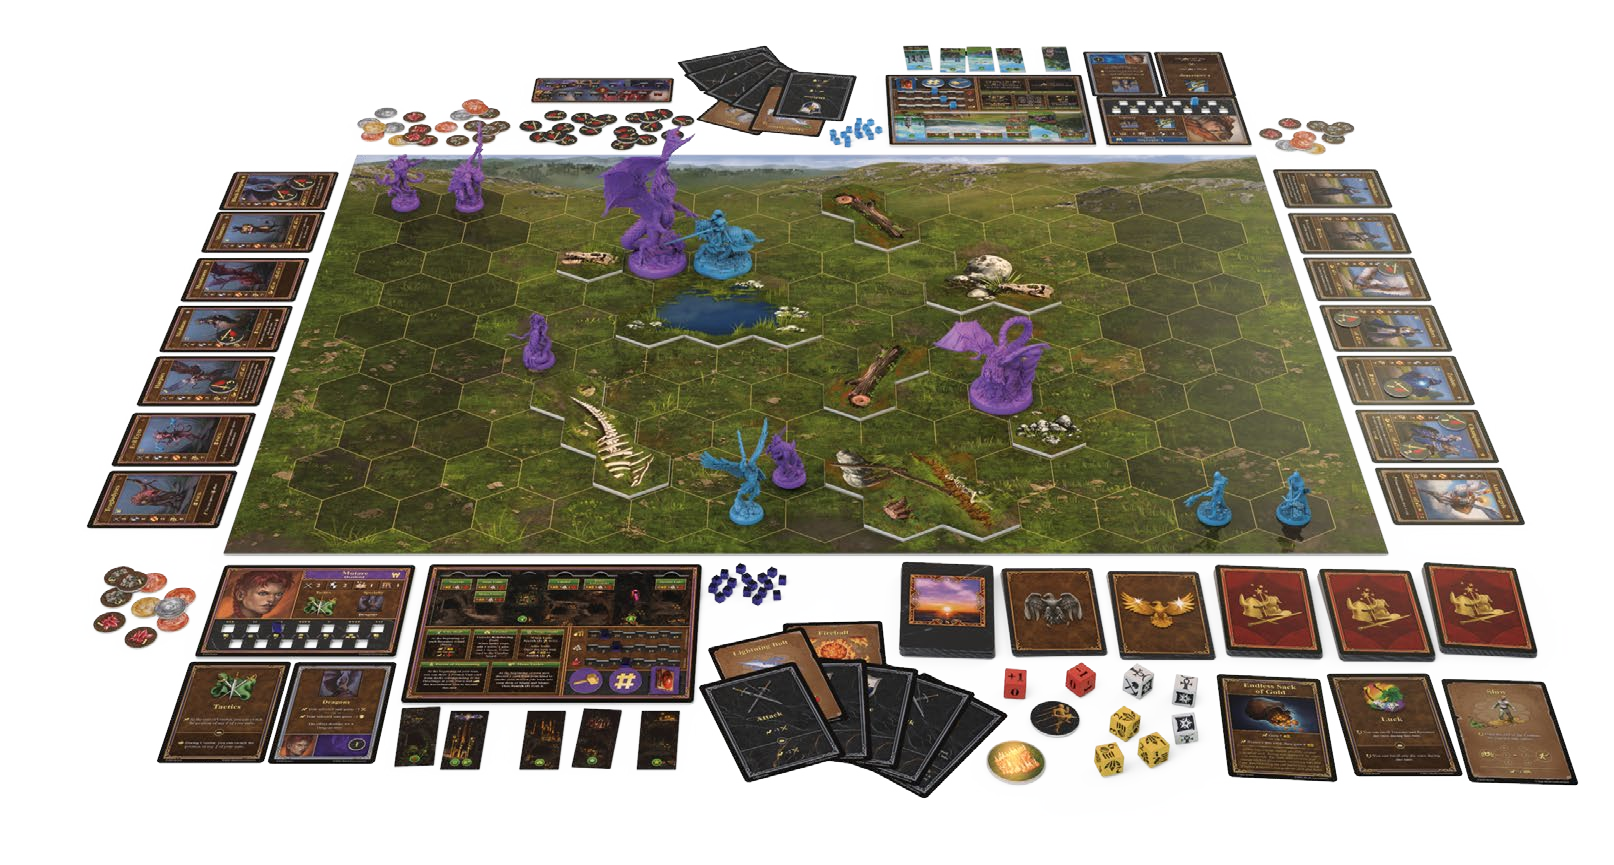
\includegraphics[width=0.9\linewidth]{\images/battlefield.png}
\end{center}
